\section{Differenzialrechnungen}
\subsection{Differenzierbarkeit}
Beide $f'_1$ und $f'_-$ müssen existieren und gleich sind.
\[ \lim\limits_{h \rightarrow 0^+} \frac{f(x + h) - f(x)}{h} \eqi \lim\limits_{h \rightarrow 0^-} \frac{f(x + h) - f(x)}{h} \]

\subsubsection{Differential}\label{differential}
Das Differential ist $dy = f'(x) \cdot dx$ und kann mit $\underbrace{f(x) - f(x_0)}_\text{dy} = f'(x_0) \cdot \underbrace{(x - x_0)}_\text{dx}$ berechnet werden. (Siehe \bronstein{444})

\subsection{Ableitungsregeln \bronstein{446}}


{\setlength{\extrarowheight}{4pt}
\begin{tabular}{@{}lcl@{}}
	\textbf{f(x)} & $\rightarrow$ & \textbf{f'(x)} \\
	\toprule
	$c$ & $\rightarrow$ & $0$ \\
	$x^n$  & $\rightarrow$ & $n\cdot x^{n-1}$ \\
	$c\cdot g\left(x\right)$  & $\rightarrow$ & $c\cdot g'\left(x\right)$ \\
	$e^x$  & $\rightarrow$ & $e^x$ \\
	\midrule
	$g\left(x\right)+h\left(x\right)$  & $\rightarrow$ & $g'\left(x\right)+h'\left(x\right)$ \\
	$u\left(x\right)\cdot v\left(x\right)$  & $\rightarrow$ & $u'\left(x\right)\cdot v\left(x\right)+u\left(x\right)\cdot v'\left(x\right)$ \\ 
	$\frac{u\left(x\right)}{v\left(x\right)}$  & $\rightarrow$ & $\frac{u'\left(x\right)\cdot v\left(x\right)-u\left(x\right)\cdot v'\left(x\right)}{v^2\left(x\right)}$ \\
	$u\left(v\left(x\right)\right)$  & $\rightarrow$ & $u'\left(v\left(x\right)\right)\cdot v'\left(x\right)$ \\
	\midrule
	$\cos\left(x\right)$ & $\rightarrow$ & $-\sin(x)$ \\
	$\sin\left(x\right)$ & $\rightarrow$ & $\cos(x)$ \\	
	$\cosh\left(x\right)$ & $\rightarrow$ & $\sinh(x)$ \\
	$\sinh\left(x\right)$ & $\rightarrow$ & $\cosh(x)$ \\
	$\tan\left(x\right)$ & $\rightarrow$ & $\frac{1}{\cos^2(x)} = 1 + \tan^2(x)$ \\	
	$\ln\left(x\right)$ & $\rightarrow$ & $\frac{1}{x}$ \\
	$f^{-1}\left(x\right) {\scriptscriptstyle (Umkehrf.)}$  & $\rightarrow$ & $\frac{1}{f'(f^{-1}(x))}$ \\
	$\left|x\right|$ & $\rightarrow$ & $\frac{\left|x\right|}{x}$ \\
\end{tabular}
}

\subsection{Tangentengleichung}
Bestimmen der Steigung $m$ durch $f'$ und anschliessend mit gegebenem Punkt $(x,y)$ folgenden Gleichung nach $b$ lösen:
$y = mx + b$

\subsection{Taylor-Reihe \bronstein{484}}
Das Tayler-Polynom approximiert eine Funktion um einen Entwicklungspunkt $a$:
\begin{align*}
	Tn(x, a) &= \sum\limits_{k = 0}^{n}\frac{f^{(k)}(a)}{k!}(x - a)^k \underbrace{+ R_n}_{\text{Restglied}}\\
	         &= f(a) + \frac{f'(a)}{1!}(x - a)^1 + \frac{f''(a)}{2!}(x - a)^2 + \dots
\end{align*}

\subsubsection{Linearisierung}
Spezialfall von Tayler-Polynom mit Entwicklungspunkt $a$:
\[\hat{f}(x) = f(a) + f'(a)\cdot(x - a)\]

\subsubsection{Restglied $R_n$}
\begin{tabular}{ll}
	Lagrange $R_n$ &= $\frac{f^{n + 1}(\xi)}{(n + 1)!} \cdot (x - a)^{n+1}$\\
	Couchy $R_n$ &= $\frac{f^{n + 1}(\xi)}{n!} \cdot (x - a)^{n+1} (1 - \beta)^n$
\end{tabular}


\subsubsection{Fehlerabschätzung}
\textbf{Absoluter}-Fehler: Maximum von gegebenem Intervall $I$ in $\left|R_n(x)\right|$ ($x \in I$) einsetzen. Achtung: Maximum variiert ja nach Funktion $f(x)$! Für $\xi \in [x, a]$ muss auch das Maximum gewählt werden, jedoch nur im Intervall von Entwicklungspunkt $a$ und gewähltem $x$.\\

\noindent Eine Funktion kann durch $R_n(x) = f(x) - T_n(x)$ gefunden werden.\\

\noindent\textbf{Relativer}-Fehler: $r = \frac{\text{absolut}}{f(x)} \rightarrow [\%]$

\subsection{Fehlerrechnung und Fortpflanzung}
\todo{Verbessern und Verallgemeinern}
Durch Substituieren von \verweiseref{differential}:
\[
\dfrac{dy}{y} = \text{Relativer Inputfehler} = \dfrac{f'(x)dx}{y} \xRightarrow[Ziel]{}\dfrac{dx}{x}
\]

\subsubsection{Mittelwertsatz Differentialrechnung}
Bei einer Sekante (Mittlerer Durchschnitt von $a$ und $b$) gibt es auf der Funktion $f$ mindestens eine Punkt mit der selben Steigung $D$. Der Punkt kann durch das Maximieren der Hilfs-Funktion $h(x)$ gefunden werden. Auch gilt der Zusammenhang von $f'(\xi) = f'(x)$!
\begin{center}
	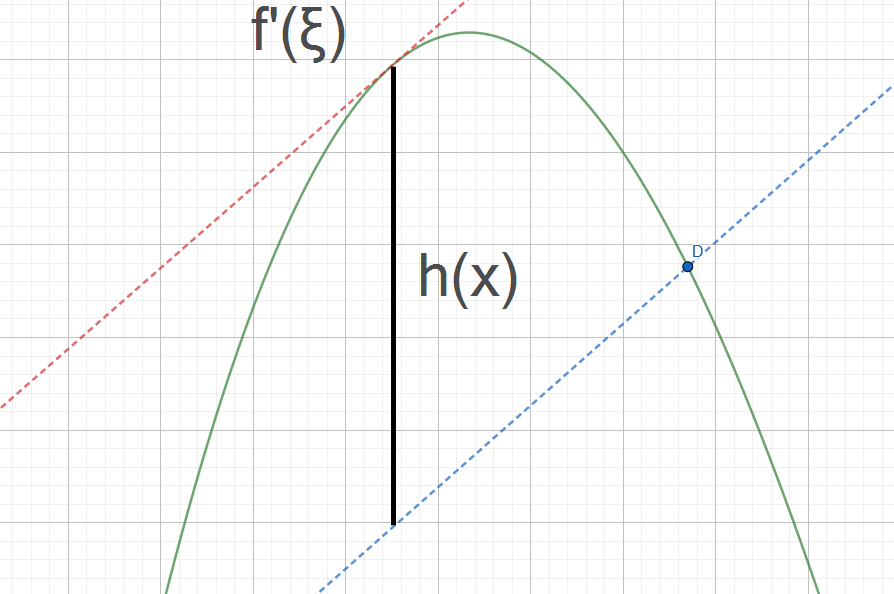
\includegraphics[height=12em]{./Images/Mittelwertsatz.png}
\end{center}

\subsection{Extremalwerte}
Um ein relative Extremalwert zu berechnen, muss die Steigung an $x_0 = 0$ sein:
$ f'(x_0) = 0 $ 
\noindent
Ob dieser Punkt nun ein Max,Min oder Sattelpunkt ist, kann die n-te Ableitung berechnet werden. \\Für \textbf{n-te Ableitung} Gerade ($2,3,\dots$) stimmt folgendes:
\[f^{(n)}(x_0) = \left\lbrace   \begin{array}{r@{}l}
	< 0 &\quad \text{Berg/relative. Maximum} \\
	> 0 &\quad \text{Tal/relative. Minimum} \\
	= 0 &\quad \text{Sattelpunkt oder \textbf{nächste Ableitung}!}
\end{array}\right.
\]
Wenn \textbf{n Ungerade} ($3, 5, \dots$) ist es ein Sattelpunkt. Falls auch $0$, nächste Ableitung


